%%% he main file. It contains definitions of basic parameters and includes all other parts.

%% Settings for single-side (simplex) printing
% Margins: left 40mm, right 25mm, top and bottom 25mm
% (but beware, LaTeX adds 1in implicitly)
%\documentclass[12pt,a4paper]{report}
%\setlength\textwidth{145mm}
%\setlength\textheight{247mm}
%\setlength\oddsidemargin{15mm}
%\setlength\evensidemargin{15mm}
%\setlength\topmargin{0mm}
%\setlength\headsep{0mm}
%\setlength\headheight{0mm}
% \openright makes the following text appear on a right-hand page
%\let\openright=\clearpage

%% Settings for two-sided (duplex) printing
% urcite tiskni oboustranne, jednostranny bakalarky jsou fuj.
\documentclass[12pt,a4paper,twoside,openright]{report}
%
% btw haha, tady si ruzny matfyzaci mysleli ze umej typografii lip nez
% profesionalove co se tim zabejvaji poslednich 300 let. Kdyby ti prislo ze
% stranky jsou tedka "divne rozjety do stran", tak to je dobre a kazdej tiskar
% to pochvali. Pak nekdy kdyztak vysvetlim proc to tak je.
%
%\setlength\textwidth{145mm}
%\setlength\textheight{247mm}
%\setlength\oddsidemargin{14.2mm}
%\setlength\evensidemargin{0mm}
%\setlength\topmargin{0mm}
%\setlength\headsep{0mm}
%\setlength\headheight{0mm}
\let\openright=\cleardoublepage

%% Prefer Latin Modern fonts
\usepackage{lmodern}

%% Further useful packages (included in most LaTeX distributions)
\usepackage{amsmath}        % extensions for typesetting of math
\usepackage{amsfonts}       % math fonts
\usepackage{amsthm}         % theorems, definitions, etc.
\usepackage{bbding}         % various symbols (squares, asterisks, scissors, ...)
\usepackage{bm}             % boldface symbols (\bm)
\usepackage{graphicx}       % embedding of pictures
\usepackage{fancyvrb}       % improved verbatim environment
\usepackage[numbers]{natbib} % citation style AUTHOR (YEAR), or AUTHOR [NUMBER]
\bibliographystyle{plainnat} % this must be moved here for natbib to work correctly
\usepackage[nottoc]{tocbibind} % makes sure that bibliography and the lists
			    % of figures/tables are included in the table
			    % of contents
\usepackage{dcolumn}        % improved alignment of table columns
\usepackage{booktabs}       % improved horizontal lines in tables
\usepackage{paralist}       % improved enumerate and itemize
\usepackage[usenames]{xcolor}  % typesetting in color
\usepackage{url}

\usepackage[textsize=tiny]{todonotes} %visual todo!

\usepackage{xspace}         %for......xspace.
\usepackage{fancyvrb}

\usepackage{pgfplots}
\pgfplotsset{compat=1.8}
\usepgfplotslibrary{statistics}


%% Generate PDF/A-2u
\usepackage[a-2u]{pdfx}

\usepackage{cleveref}       %\cref yay!

%% Character encoding: usually latin2, cp1250 or utf8:
\usepackage[utf8]{inputenc}

%%% Basic information on the thesis

% Thesis title in English (exactly as in the formal assignment)
\def\ThesisTitle{Efficient simulation of environment destruction in games}

% Author of the thesis
\def\ThesisAuthor{Marek Dobranský}

% Year when the thesis is submitted
\def\YearSubmitted{2017}

% Name of the department or institute, where the work was officially assigned
% (according to the Organizational Structure of MFF UK in English,
% or a full name of a department outside MFF)
\def\Department{Department of Software Engineering}

% Is it a department (katedra), or an institute (ústav)?
\def\DeptType{Department}

% Thesis supervisor: name, surname and titles
\def\Supervisor{Mgr. Miroslav Kratochvíl}

% Supervisor's department (again according to Organizational structure of MFF)
\def\SupervisorsDepartment{The Department of Software Engineering}

% Study program and specialization
\def\StudyProgramme{Computer Science}
\def\StudyBranch{Programming and Software systems}

% An optional dedication: you can thank whomever you wish (your supervisor,
% consultant, a person who lent the software, etc.)
\def\Dedication{%
I would like to express my gratitude to Mgr. Miroslav Kratochvíl, the supervisor of this thesis, for his patient guidance, feedback and all advice he has given me. 

I also want to thank my family and girlfriend for their continued support and encouragement during my Bachelor studies and especially during the time spent working on this thesis.
}

% Abstract (recommended length around 80-200 words; this is not a copy of your thesis assignment!)
\def\Abstract{%
Destructible environments have become a popular feature of computer games. Currently used game engines employ different approaches to implement such environment. This thesis studies several such approaches and implements some key ideas from available research in a new, combined approach. We use tessellations and boolean operations on triangular meshes to modify rigid-body objects that represent game environment, and create a simple application to demonstrate the approach in a real-time environment. We conclude that the proposed method is mainly suitable for computer games that feature low-polygon meshes.
}

\def\AbstractSK{
Deštrukcia v hernom prostredí sa stala populárnou súčasťou počítačových hier. Aktuálne používané herné enginy využívajú rôzne prístupy k deštrukcii. Táto práca študuje niekoľko takýchto prístupov a implementuje vybrané kľúčové myšlienky z dostupných štúdií, v novom kombinovanom prístupe. Používame delenie objektov a boolovské operácie na trojuholníkových sieťach k modifikácii pevných objektov, ktoré reprezentujú herné prostredie a tiež tvoríme jednoduchú aplikáciu k demonštrácii vybraného prístupu v reálnom čase. Dospeli sme k názoru, že navrhnutá metóda je použiteľná najmä v počítačových hrách so sieťami s malým počtom mnohouholníkov.
}

% 3 to 5 keywords (recommended), each enclosed in curly braces
\def\Keywords{%
destructible environment, simulation, games, convex decomposition, polygon mesh
}

%% The hyperref package for clickable links in PDF and also for storing
%% metadata to PDF (including the table of contents).
%% Most settings are pre-set by the pdfx package.
\hypersetup{unicode}
\hypersetup{breaklinks=true}

% Definitions of macros (see description inside)
\include{macros}

% Title page and various mandatory informational pages
\begin{document}
\include{title}

%%% A page with automatically generated table of contents of the bachelor thesis
\tableofcontents
%%% Each chapter is kept in a separate file
\chapter*{Introduction}
\addcontentsline{toc}{chapter}{Introduction}
\todo {text here}
%Taky pozor na to, ze do Introduction je tradicne taky potreba dat nejaky "related work" kde tyhlety clanky jen rychle shrnes, aby si oponent moh rychle predstavit kde presne ta bakalarka mezi nima lezi.

\begin{itemize}
\huge \color{red}
\item abstract - waiting for corrections
\item intro - TODO
\item 1 - DONE
\item 2 - waiting for corrections
\item 3.1-3.4 - DONE
\item 3.5 - waiting for corrections
\item conclusion - TODO
\end{itemize}

\chapter{Overview of techniques}
This chapter introduces the techniques used to simulate destructible environments. First, we talk about the development of the destructible environment in several games and game engines, then about general approaches to this problem.

We will repeatedly categorise the content of the game world in following way: We will use the word \emph{object} to refer to any building, crate, door, tree or other items that occur in the game environment, but excluding terrain, distant environment like skyboxes and any in-game characters. Most of the modern 3D games use the term destructible environment as a reference to destructible objects because they do not support the destruction of terrain. We will comply with this terminology and, unless specified otherwise, use the term destructible environment as a reference to a destruction of game objects and not the terrain.

\section{Implementations in mainstream gaming}
\label{sec:common}
In this brief overview, we introduce the most common approaches to environment destruction that can be seen through the games released in last 40 years. More common approaches can be seen used in newly released games.

\para{Object replacement or removal} was the first~\cite{history} method used to simulate a destructible environment in a computer game, mostly because it is straightforward and undemanding. This approach is based on swapping models or any other kind of visual representations, for more damaged ones or completely removing them. Because it relies on pre-made models, exact collision points on the models are not considered, and the result is always the same. If we were to consider $N$ points of taking damage, the number of different models could grow up to $2^N$. A large number of models is not practical for game development, other approaches are therefore used for breaking the object at the precise point. Despite its simplicity and limitations, this approach can still produce a very desirable result. In fact, it is still most widely used approach to a destructible environment in computer games.

In our simplified view on 2D games, we will not differentiate between objects and terrain and refer to both as the environment.
First 2D games featuring the destructible environment were arcade games like the \emph{Space Invaders (1978)}\footnote{\url{https://en.wikipedia.org/wiki/Space\_Invaders}} where the environment is represented by cells in a grid. After taking damage, the visual representation of the cell is replaced by one looking more damaged and the finally completely removed. About a decade later, new environment destruction technique was used in games like \emph{Scorched Earth (1991)}\footnote{\url{https://en.wikipedia.org/wiki/Scorched\_Earth\_(video\_game)}} and \emph{Worms (1995)}\footnote{\url{https://www.team17.com/games/worms-original}}. Collision and removal of terrain in those games is based on individual pixels rather than whole objects, which creates a more realistic visual effect. In \emph{Scorched earth} players typically need to blow away a hill dividing them, in \emph{Worms} it is common to dig a tunnel to hide from your enemies gunfire.

In 3D games, the principal technique of implementation of destructible objects has not changed much over the years. For every object that the player can modify there is a prepared set of alternative models with various amount of damage applied. Based on how much damage is applied, the models are swapped and eventually completely removed, as seen in \cref{fig:doors}. Swapping the models is usually accompanied by animations, debris and dust generation, designed to hide the unrealistically instant change of the object from the player. The disadvantage of this method is the necessity to replace the in-game objects as a whole --- there has to be a significant number of objects pre-made for different scenarios to make the game look realistic. A small number of pre-made damaged models means this approach can not flexibly react to specific player actions. As an example, in the \emph{Source} engine, the hole in the door (\cref{fig:doors}) is always created at the same place, regardless of the point of the impact. Another example can be found in the game \emph{Duke Nukem 3D}\footnote{https://en.wikipedia.org/wiki/Duke\_Nukem\_3D}, where specific parts of the walls are created as separate objects that disappear when hit.

\begin{figure} 
\centering
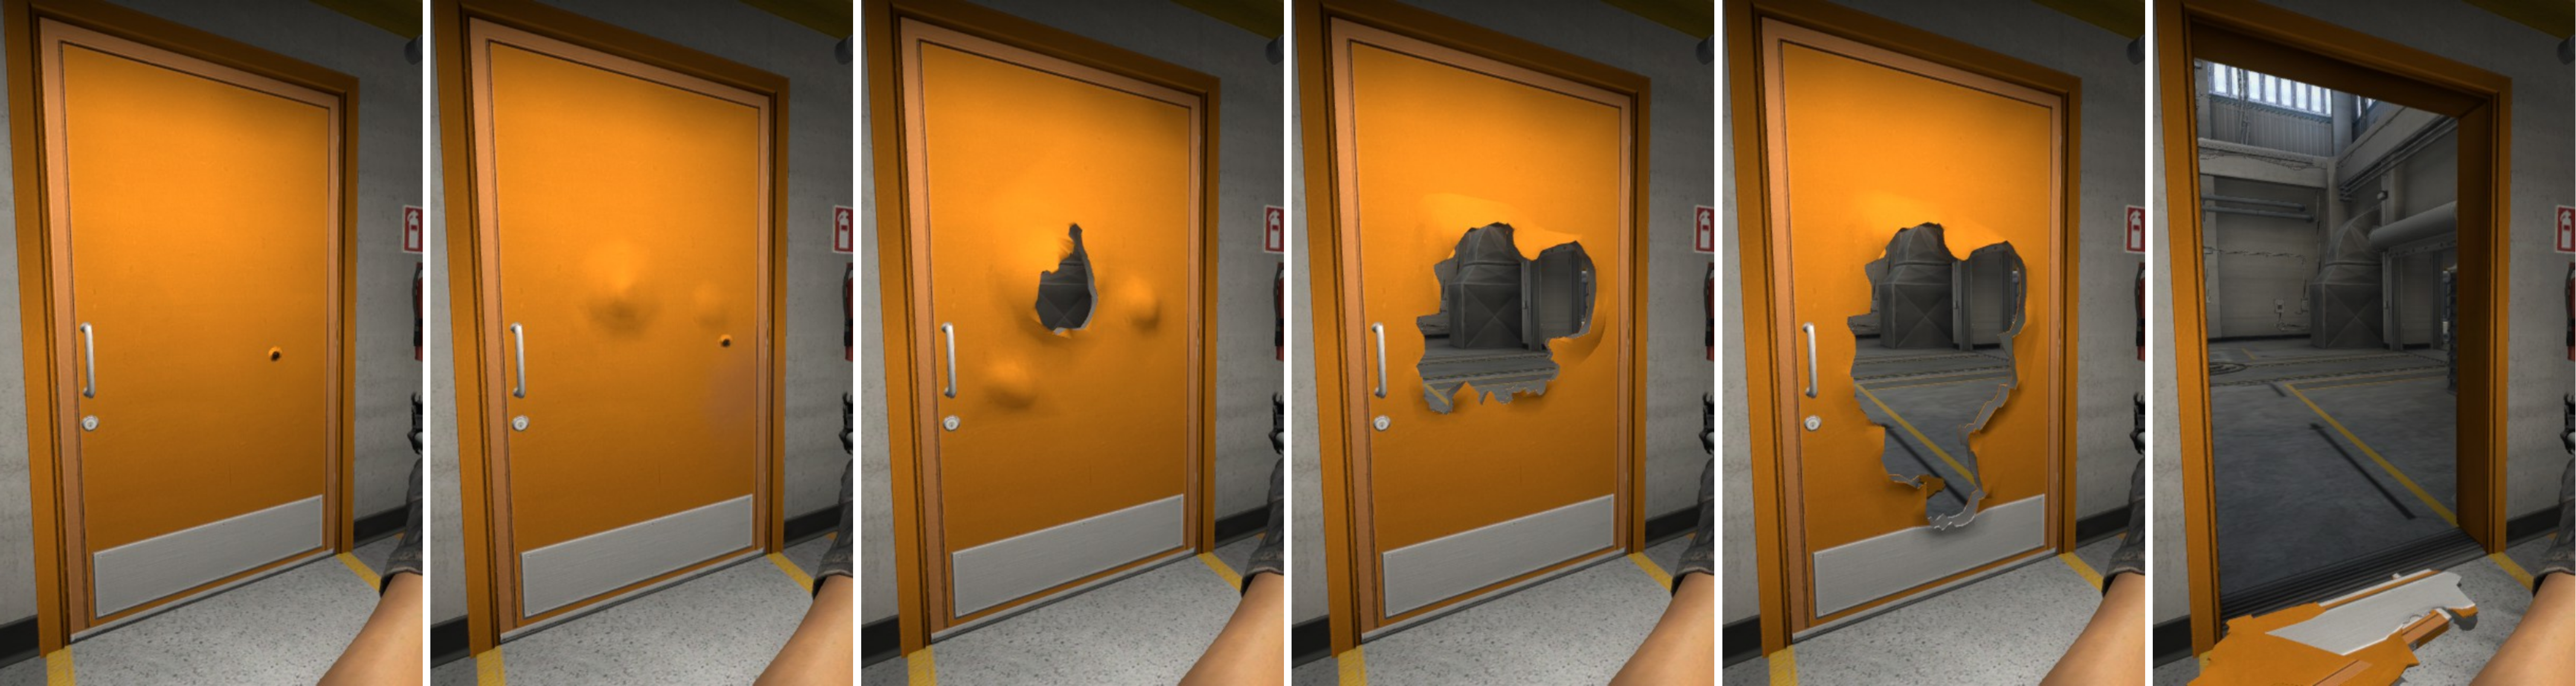
\includegraphics[width=\textwidth]{img/doors}
\caption{\emph{Source} engine swaps door models. Image taken from \emph{Counter Strike: Global Offensive}. Successively damaging any doors in the game will always produce this sequence of models, regardless of the exact point where the damage was applied.}
\label{fig:doors}
\end{figure}

\para{Height map approach} is closely intertwined with terrain generation. The basic principle behind modifying the environment with this method is changing the height of the terrain at given point. We can find this method used in the first 3D games that featured destructible terrain, \eg \emph{Magic Carpet (1994)}~\footnote{\url{https://ultimatehistoryvideogames.jimdo.com/magic-carpet}} or \emph{Starfighter 3000 (1994)}~\footnote{\url{https://en.wikipedia.org/wiki/Star\_Fighter\_(video\_game)}}.

The height map of a 3D terrain is defined as a uniform 2D grid of values representing height of their respective column in 3D space. A convenient approach is to use 2D grey-scale bitmap and represent the height as a colour distance from the white colour, black being the maximum. Because the grid only contains information about the discrete points, interpolation is used to create continuous terrain. We can also view this method as creating a function of two coordinates on the plane giving us the value on the vertical axis. The definition of function forbids more than one function value at each input point, therefore this method can not represent multiple layers of terrain. The relative simplicity of the approach is counterweighted by the fact that it can only change the height of the terrain and does not allow creating caves, tunnels or similar hollow features.

\para{\emph{Geo-Mod}} (\emph{Geometry Modification Technology}\cite{geomod}) is an engine developed for the \emph{Red Faction (2001)}\footnote{\url{http://redfaction.wikia.com/wiki/Red\_Faction}} video game. It approaches the modification of the terrain by creating objects representing a empty space. After every collision, a new object is created at the point of collision. This new object is then subtracted from the terrain creating the modified terrain with the newly created hole. The difference of the meshes is calculated in real time. Game reviews suggest, the engine does not work well with the buildings and other objects. \emph{Geomod} represented the first significant attempt to create the fully destructible 3D environment that would work under real-time constraints.

\para{\emph{Geo-Mod 2}}~\cite{geomod}\footnote{Geo-Mod 2.0 presentation video \url{https://www.youtube.com/watch?v=lICurOVsNv0}} does not feature destructible terrain, instead, it focuses on realistic destruction of buildings. A set of smaller objects is used to represent each building as a ragdoll (multiple objects connected with joints) for the simulation of inner stresses. Switching from using a conventional 3D model to the ragdoll simulations, requires at least basic knowledge of civil engineering in order to properly analyse structural stability of the building and create a ragdoll model simulating it properly. This process is done by hand in the development process and can not be modified at a runtime. The high complexity of simulation limits the engine in the scale of the game world and mutual proximity of destructible objects. Because of that, game avoids any interaction of multiple buildings requiring simulating their behaviour at once.


\para{\emph{Frostbite}}~\footnote{http://www.frostbite.com/about/frostbite-3} engine (and mainly its component \emph{Destruction}~\cite{destruction}) is currently used in new mainstream games that feature destructible environment \eg \emph{Battlefield} series or \emph{Star Wars Battlefront (2015)}. It supports two different kinds of destruction micro-destruction on the surface and the large scale predetermined destruction on whole buildings. 

The dynamic micro-destruction focuses on creating small dents into the surface of the object. The dents are created dynamically at the point of impact and can be placed on any point of the surface.

The large-scale destruction is focused on destroying entire buildings. The buildings are created from smaller parts that are linked together. Each part can disappear on its own (\cref{fig:frostbite}), and when there is not enough parts left, the whole building collapses. It does not use any physical simulation in this process and therefore structural stability is determined solely from the number of removed parts of the building.

\begin{figure}
\centering
\includegraphics[width=\textwidth]{img/frostbite}
\caption{The arrangement of destructible elements for the large-scale destruction in \emph{Frostbite} engine (on the left). Rest of the images shows the process of large-scale destruction in \emph{Battlefield: Bad Company} implemented using \emph{Frostbite 1}.}
\label{fig:frostbite}
\end{figure}

\section{Methods and algorithms}

Here we will give a short overview of several more rigorous algorithms commonly used for simulations of destructible environment. 

In simulations, we consider two types of objects: soft bodies and rigid bodies. A rigid body represents an object with a constant shape where every two points on the body are always in the same relative position. On the other hand, soft bodies are deformable under an applied force, meaning a point on the body can change its position independently on every other point. Although there are no actual rigid objects in the real world, soft body simulation is computationally more expensive than the rigid body one. Therefore, in the computer games, rigid body simulation is used almost exclusively. Although we so not perform soft body simulations, we try tu emulate them in real-time on rigid bodies.

When trying to save a processing power, there is another way to do it on soft bodies. Many soft bodies are non essential to the gameplay and their simulation would not bring more value to the game \eg waving flag or flowing water. Those bodies can be implemented as a pre-rendered animations and not actual simulations.

\subsection{Soft body deformation}
In this section, we will shortly introduce two different approaches for simulation of soft bodies. Despite the fact that soft bodies are currently rarely used in computer games to the extent of destructible environment, a several soft body objects can show up in a game. We also expect that with an evolution of more powerful hardware, soft body deformation will make its way into the gaming world \eg \emph{Next Car Game: Wreckfest (2018)}~\footnote{\url{http://store.steampowered.com/app/228380/Next\_Car\_Game\_Wreckfest/}} will use soft bodies to simulate car crashes.
\label{sec:softBody}

\para{Finite Element Method} (FEM) is a numerical method used to simulate the behaviour of a system that can be modelled by solving the behaviour of the smaller discrete parts, called finite elements. Each element calculates its physical state, \eg stress or temperature, and propagates the results to neighbouring elements. This model can be used for simulation of fluid dynamics, brittle fractures~\cite{brittlefracture}, ductility~\cite{ductilefracture}, elasticity, heat transfer and other physical properties. It is beneficial in engineering, modelling and rendering scenes for computer generated images ~\cite{Bargteil:2007:AFE}. 

FEM requires a lot of computational resources and is mostly used in simulations that are not in real-time constraints. The algorithms like \citet{femingames} propose, that optimised version of FEM can be used in computer games.


\para{Material point method} (MPM) is a numerical method for modelling an object as a continuum mass. Continuum model assumes that the object completely fills the space it occupies and is not a set of discrete particles. MPM is able to simulate such materials by using two different views of the data, material points (Lagrangian elements) and Eulerian grid. MPM is a particle method but thanks to the Eulerian grid it can by applied to continuum materials. 

MPM is more computationally expensive than FEM, as the grid must be reset at the end of each MPM calculation step and reinitialised at the beginning of the following step. On the other hand MPM is a meshfree method and does not require remeshing steps. 

MPM works by projecting the data from the particles to the mesh, determining and applying the velocities on the nodes of the mesh and then updating the particles based on the deformation of the mesh. After each loop mesh needs to be reset while the data stay in particles.

 A simplified overview of algorithm steps follows, for more details see the thesis of \citet{jiang2015material}.
 
\begin{enumerate}
    \item Grid data are reinitialized to default values.
    \item Weights and weight gradients are computed on every particle.
    \item Mass and momentum are transferred from the particles to the grid.
    \item The explicit forces on nodes are calculated
    \item The explicit nodal velocity update is performed
    \item Grid based collision is performed on vertices.
    \item Particles are updated from grid velocities.
\end{enumerate}
These steps are illustrated in \cref{fig:mpm}.

MPM is useful for both fluid and soft body dynamics. It can simulate deformation, fractures, heat transfer, melting and other changes of the state of an object.

A popular example of MPM deployment can be seen in snow simulation in the \emph{Disney} film \emph{Frozen (2013)}. The simulation software \emph{Matterhorn}\footnote{https://www.disneyanimation.com/technology/innovations/matterhorn} computes the behaviour of different types of snow (\eg wet, fresh, sticky) and other materials, such as sand or mud.

\begin{figure}
\centering
\includegraphics[width=\textwidth]{img/MPM}
\caption{Material point method algorithm overview. The top and the bottom rows operate in particle domain (Lagrangian) while the middle depicts grid-based (Eulerian) operations \cite{disney}.
}
\label{fig:mpm}
\end{figure}

\subsection{Rigid body decomposition}
In the soft body, application of the force propagates across the particles, and the connected particles break apart when the limit is exceeded. This creates the fracturing that may lead to the whole body splitting. In the rigid body simulation, the body has no internal structure, and therefore the applied force can only change the momentum of the entire body. This prohibits the deformation or fracturing a rigid body in a simulation.

To solve this problem, there are numerous approaches of decomposing the rigid body in the way that imitates fractures achieved by exceeding the elasticity of the soft material. The most common approach is a decomposition of a rigid body into smaller parts. Some of the common methods for decomposition are: slicing by planes~\cite{minettooptimal}, convex decomposition~\cite{Lien:2007:ACD:1236246.1236265}, tetrahedralization~\cite{frey1996delaunay} and Voronoi tessellation. In this section we will describe a process of Voronoi tessellation.

Voronoi tessellation is a method of decomposing a solid object into smaller parts, as shown on \cref{fig:voro}. It is also applicable for \eg terrain generation~\cite{voronoiterrainrealtime}, but we will focus on object decomposition. Assuming the input is a closed triangular mesh with non-empty volume, the tessellation can be done in following three steps:

\begin{figure}
        \centering
        \includegraphics[width=0.5\textwidth]{img/clippedresult}
        \caption{The result of Voronoi tessellation \cite{yan2010efficient}}
        \label{fig:voro}
\end{figure}

\begin{description}
    \item[Delaunay tetrahedral decomposition] Given points $P$ in general position (the vertices of input mesh and a set of points inside its volume), tetrahedral mesh $DT(P)$ can be generated satisfying the following condition: no point in $P$ is inside the circumscribed sphere of any tetrahedra in $DT(P)$~\cite{cignoni1993parallel}.
    \item[Creating Voronoi diagram] For a Delaunay tetrahedral decomposition, its dual graph (with vertices in the centre of tetrahedrons circumscribed sphere) is a Voronoi diagram (see \cref{fig:voro}).
    
 \begin{figure}
    \centering
    \includegraphics[width=0.4\textwidth]{img/delaunay}
    \includegraphics[width=0.4\textwidth]{img/voronoi}
    \caption{Transformation of 2D Delaunay triangulation to Voronoi diagram. Source: \url{https://en.wikipedia.org/wiki/Delaunay\_triangulation}}
    \label{fig:DT}
\end{figure}

    \item[Clipping the Voronoi diagram] Boundary cells of the Voronoi diagram are infinite (see \cref{fig:DT}) and need to be clipped by the original input triangular mesh. The efficient algorithm proposed by~\citet{yan2010efficient} for this task finds the intersection of the boundary Voronoi cell with the triangular mesh and continues with neighbourhood propagation to determine all intersections. 
\end{description}

 \begin{figure}
    \centering
    \includegraphics[width=\textwidth]{img/clipped}
    \caption{Timing curve of clipped Voronoi diagram computation against the number of Voronoi seed points on a model with 1000boundary triangles.  To achieve clipped Voronoi diagram all three tasks must be completed. Source: \citet{yan2010efficient}}
    \label{fig:vorocliptime}
\end{figure}

As we can see in the performance diagram~\cref{fig:vorocliptime} the Voronoi tessellation with hundreds of thousands of Voronoi sites can take number of seconds to calculate. However, for a destructible environment hundreds of pieces will suffice, therefore this method can be used in a real-time application.  

\section{Related research}
In this section we review two results of recent research that propose different techniques for environment destruction in computer games. First technique focuses on simulating the forces inside the object with the approach based on particle methods. The second one focuses solely on the destruction of rigid bodies with the use of Voronoi decomposition.

\subsection{A fast method for simulating destruction and the generated dust
and debris}
\label{sec:edem}
The method of \citet{edem} approaches destruction on three scales. At first, the destruction is performed on a coarse scale, and then the applied energy is used to calculate the amount and size of smaller debris and finally dust particles.

\begin{description}
\item[Destruction on a coarse scale] on this level the authors use Extended Distinct Element Method (EDEM) which is based on Element Method described in section \ref{sec:softBody}. Instead of using particles, EDEM uses a set of rigid bodies that need to be produced by some tessellation method. The extension over traditional DEM is the use of pore springs to connect the adjacent elements (see \cref{fig:spring}). The authors compare the elements to individual bricks (the distinct elements) held together by layers of mortar (the pore springs). If the applied force is sufficient to move the elements far enough from each other, the fracturing process is initiated. Pore springs also help the object retain its original shape after the force is applied. 
\begin{figure}[t]
        \centering
        \includegraphics[width=0.7\textwidth]{img/spring}
        \caption{The force between two EDEM elements \cite{edem}}
        \label{fig:spring}
\end{figure}
\\Algorithm for creating EDEM elements
\begin{enumerate}
\item Represent the original object as a closed surface model.
\item Arbitrarily arrange the EDEM elements inside the object.
Elements are allowed to overlap at this point.
\item Move elements by performing the EDEM simulation. Only the contact force will be considered in this simulation.
\item Perform collision detection between the object’s surface
and elements, making sure that they always
stay inside the object.
\item Repeat (3)–(4) until elements are stabilised.
\item Construct a Delaunay diagram from the set of elements
and put the pore springs on the Delaunay edges that connect
the elements
\end{enumerate}
We can see the distribution of the EDEM elements inside objects after collision on \cref{fig:edem}.

The position $\mathbf{x}_I$ and velocity $\mathbf{v}_I$ of the element $\mathit{I}$ can be found using Newton’s equation of motion as follows:
 
\[M\frac{d\mathbf{v}_I}{dt} = \sum_{J \in contact}^{} \mathbf{F}_{JI}^c + \sum_{K \in pore}^{} \mathbf{F}_{KI}^p + M\mathbf{g} \]
\[ \frac{d\mathbf{x}_I}{dt} = \mathbf{v}_I \]
Here, $\mathbf{g}$ is the gravitational vector, $\mathbf{F}^c_{JI}$ is the contact force, $\mathbf{F}^p_{KI}$ is the force due to the pore springs and $\mathit{M}$ is the element’s mass. Two elements \{I, J\} are in contact, if they are closer to each other than the diameter of a single element.

\item[Fine debris generation and simulation] If a fracture between EDEM elements happened, we can determine if there was enough energy to break EDEM element into smaller debris. The probability distribution is used to determine the size of debris. Debris is taken out of EDEM simulation and put into particle simulation, where each piece is represented as a particle without volume.

\item[Dust generation and simulation] Amount of generated dust is based on fracture energy and results of debris generation. Instead of simulating particles smaller than predetermined margin, they are represented as dust in a grid-based fluid simulation. The density of particular cell represents the amount of dust.

\end{description}

 \begin{figure}
        \centering
        \includegraphics[width=0.49\textwidth]{img/edem_real}
        \includegraphics[width=0.49\textwidth]{img/edem}
        \caption{View of final rendering with generated dust and debris (left) and equivalent view showing underlying EDEM elements (right) \cite{edem}}
        \label{fig:edem}
    \end{figure}
   
\begin{table}[ht!]
    \begin{center}
  \begin{tabular}{cc} 
  \parbox[b]{4em}{\centering EDEM\\elements} & FPS \\
  \hline
  128 & 320 \\
  256 & 160 \\
  512 & 75 \\
  1024 & 30 \\
  2048 & 9.1 
  
  \end{tabular}
  \end{center}
  \caption{Performance of EDEM element method without rendering \cite{edem}}
  \label{table1}
\end{table}
In conclusion, based on \cref{table1}, the frames per second (fps) drop proportionally with growing number of EDEM elements. The method achieved interactive fps on moderate number of EDEM elements. In addition, the proposed debris and dust generation can be combined with other methods.


\subsection{Real Time Dynamic Fracture
with Volumetric Approximate Convex Decompositions}
\label{sec:RTDF}
The approach of \citet{nvidia} does not try to simulate the internal forces of an object and focuses only on rigid body decomposition. The idea behind this method is to represent the mesh as a compound shape of convex parts. The algorithm used for convex decomposition is Volumetric Approximate Convex Decomposition (VACD), which works by introducing the Voronoi decomposition into a bounding box of the mesh and then clipping the Voronoi cells by the mesh. To determine the decomposed shapes, we use a prepared fracture pattern. The fracture pattern is precomputed and represented as a set of convex cells. The algorithm works as follows (the process is visualised in \cref{fig:vacdalg}:
\begin{enumerate}
\item The fracture pattern is aligned with the point of impact, and rotated and scaled randomly to avoid an occurrence of same-looking patterns.
\item The intersections of all cells with all convex parts are computed. To compute the intersection of a single cell with a single convex part, the convex part is clipped against all the planes of the cell one by one. 
At the end of this step, we have a set of new convex parts, and each convex part belongs to exactly one cell.
\item If there are convex parts that together entirely fill one cell, we can combine them into single new one convex part. The test is carried out using a simple volume comparison.
\item All convex parts that belong to one cell are combined to form a new compound part. This ensures that the temporary parts of decomposition into compound shape are not visible after the fracture (see \cref{fig:vacdfracture}).
\begin{figure}
        \centering
        \includegraphics[width=0.7\textwidth]{img/vacdfracture}
        \caption{The decomposition to the
initial compound mesh does not become visible when a fracture
pattern is applied. Source: \citet{nvidia}}
        \label{fig:vacdfracture}
\end{figure}
\item Finally, the separate islands of convex parts are detected and individual compound shapes are constructed for them.
\end{enumerate}

\begin{figure}
\centering
        \includegraphics[width=\textwidth]{img/vacdAlgorithm}
        \caption{Overview of the fracture algorithm. Left: The fracture pattern (red) is aligned with the impact location (black dot). Middle: All
convex pieces are intersected with all cells. The green convex pieces can be welded to form a single piece because they cover the entire
cell. Pieces within one cell become a new compound part (same colours). Island detection finds that the dark red compound needs to be split. Source: \citet{nvidia}}
        \label{fig:vacdalg}
\end{figure}

The cost of fracturing in this method depends only on the number of mesh triangles of the object being fractured and the resolution of fracture pattern. The paper suggests that the model with $10^6$ vertices and $5\cdot10^5$ faces can be fractured under 50ms. This makes this method suitable for real-time computer games.


\chapter{Review of related software libraries}
\label{chapt:technology}
In this chapter we introduce libraries that can be beneficial for creating a destructible environment. We do not talk about all-in-one software development kits with their own approach to destructible environment already implemented. Instead our focus is on building a game with destructible environment from zero.  

To build a game we will surely need a physics engine, a graphics engine, and to support our destructible environment a selection of geometric libraries. We mention which libraries we used in the implementation and details of their use can be found in~\cref{app:implementation}.

We committed ourselves to writing our application in \emph{C++} language and using only free software. This commitment limits us in the  availability of certain software.

\section{Physics engine}
Bullet Physics
\todo {text here}


\section{Graphics engine}
Irrlicht Engine
\todo {text here}

\section{Geometric libraries}
\todo {text here}

\subsection{Boolean operations}

When searching for efficient library able to compute the difference of two 3D triangular meshes, we found out that the majority of available software is dependent on using \textbf{The Computational Geometry Algorithms Library}~\footnote{http://www.cgal.org/} or shortly \textbf{CGAL}. CGAL provides a polyhedral surfaces that are closed for Boolean operations and it is possible to to convert data between meshes and polyhedrons. The choice to use CGAL creates restrictions on 3D meshes we can use (for more details on data structure see~\cref{app:implementation}).

We considered using a \textbf{Cork Boolean Library}~\footnote{https://github.com/gilbo/cork\#cork-boolean-library} but we did not found it to be as robust as CGAL.

\subsection{Voronoi tessellation}
We learned that to Voronoi tessellation can be beneficial to either creating a compound body held together by springs or used as a tool for subtracting parts of the mesh. Here are some libraries useful for both tasks.

\begin{description}
\item[CGAL] also includes package providing different 3D triangulations, mainly Delaunay triangulation and the possibility of creating Voronoi diagram as its dual graph. However CGAL does not provide means to clip the Voronoi cells against the surface mesh.

\item[Voro++]\footnote{http://math.lbl.gov/voro++/} is a library for carrying out three-dimensional computations of the Voronoi tessellation. It calculates Voronoi cell for each particle individually and is suited for high performance calculations on large scale particle systems. It is also able to clip Voronoi cells to any user defined boundary. This library would be well suited for decomposing whole objects into Voronoi cells. 

Because implementation requires only one Voronoi cell per collision, we chose to use the simpler Voro++ library for this task. 
\end{description}


\subsection{Convex decomposition}
\label{sec:decompositionLib}
Convex decomposition is critical to fast and accurate collision detection on 3D meshes. We introduce two libraries with different approaches to the task.
\begin{description}
\item[CGAL] provides the means for decomposing the polyhedral shape (triangular mesh can be converted into polyhedron) into a set of convex polyhedrons. CGAL is aiming for an exact convex decomposition, which produces a large number of small pieces~\footnote{http://doc.cgal.org/latest/Convex\_decomposition\_3}.

\item[Hierarchical Approximate Convex Decomposition] or HADC~\cite{HACD} is a library and algorithm providing a convex decomposition that approximates the original shape. The approximation yields less pieces and is faster than exact calculations but the result is not exact. For the reasons that we are implementing a destructible environment in a computer game, we can allow for deviations in the shape of the objects from their respective visual representations. Those deviations should be too small to be noticed in game. This makes us choose HACD over CGAL.
\end{description}

We can see the difference in the result of those two approaches on~\cref{fig:bunny}. It is obvious that we do not want to use the exact decomposition in a computer game, but on the other hand for the simulations where the calculation time is not critical the approximations should not be used.
\begin{figure}
        \centering
        \includegraphics[width=\textwidth]{img/bunny}
        \caption{Difference between original mesh, exact convex decomposition and an approximate convex decomposition. Source: https://github.com/kmammou/v-hacd}
        \label{fig:bunny}
\end{figure}



\chapter{Implementation Design}
\label{chaptImplementation}
In this chapter, we will introduce the implementation of our demo game and explain the basic principles and algorithms behind it.
\todo {mention measurements}

After consideration of the various approaches implemented in games and also proposed efficient solutions to the problem of real-time destructible environment, we decided to implement and test a combination of reviewed techniques:  Our approach is similar to \emph{Geomod} (described in \cref{sec:common}) and \emph{Real Time Dynamic Fracture with Volumetric Approximate Convex Decompositions}(RTDF) (described in \cref{sec:RTDF}), but with several key differences described below.

\section{Main algorithm}
\todo{tohle zacina trochu odprostred --- jaky sou struktury v tom algoritmu? jak reprezentujes objekty? kde se tam objevi ta kolize?}
Our approach generates Voronoi cell at the point of collision. Then the difference of original mesh and the Voronoi cell is calculated and represents the damaged object. To generate the debris, the intersection of original mesh and the Voronoi cell is calculated. This action effectively cuts the object into two or more pieces, all of which are put back into simulation and can be damaged again (see \cref{fig:subtraction}). The Voronoi cell was chosen because it has easily randomizable shape and provides aesthetically good results. This choice is in no way critical to the rest of algorithm, any other closed mesh can be used as well.

Similarly to the RTDF approach, the cost of fracturing in our implementation is solely dependent on the size and complexity of the fractured object. \todo{odkaz na merania} This makes the method suitable for use in computer games and real-time simulations. \todo{to je trosku bold claim --- urcite to nebude fungovat pro vsechny hry. Je dobry se presne vymezit --- velikost objektu do cca X polygonu, ...}

\begin{figure}
        \centering
        \includegraphics[width=\textwidth]{img/subtractionProcess}
        \caption{object with point of impact (left), generated Voronoi cell (centre), object divided into six new smaller objects after subtraction of Voronoi cell (right)}
        \label{fig:subtraction}
\end{figure}

Randomization of the size and shape of a Voronoi cell guarantees different result after every collision. The generation of a Voronoi cell takes place in a closed domain with its centre at the point of collision. In the domain, in addition to the centre point, random points need to be generated. The used Voronoi cell is the cell of the centre point cut by the boundaries of the domain if necessary.
\todo{Tadyto vysvetleni neni OK, predpoklada ze clovek uz vi jak ten tvuj algoritmus funguje a tady ho jen tak ujistujes ze to dobre chape. }

We also considered implementation based on \emph{A fast method for simulating destruction and the generated dust and debris} (see \cref{sec:edem}). To test this approach, we set up a cube divided into 439 tetrahedrons.\todo{Tohle je mereni, do designu to definitivne nepatri. Muzes sem napsat ze si svou metodu vybral experimentalne ze dvou protoze ta druha mela degraded performance, a odkazat se na mereni.} After introducing constraints to hold the tetrahedrons together, we experienced a drop from 60fps (set as an upper limit) to 13fps. Having a large number of elements connected with springs in the simulation can also trigger an undesirable behaviour, such as contractions, retractions and self-induced explosions of the object. Performance issues and problems with keeping elements in a stable state finally concluded that the approach was not suitable for our implementation.


\section{Program Structure}
Disregarding the initialization\todo{mozna rekni ze ji popises pozdejs a dej duvod proc to odkladas, neni moc dobry to zbytecne roztrhat.}, the program runs in following steps:
\begin{enumerate}
\item Perform a step in physics simulation.
\item Handle collisions and perform destruction, see \cref{sec:collisions}.
\item Read user input and then apply correct forces to controlled vehicle.
\item Render current state of objects. In this step, a graphical representation of every object is updated to comply with its rigid body version.
\end{enumerate}

\begin{figure}
        \centering
        \includegraphics[width=\textwidth]{img/decompositionFlow}
        \caption{Diagram is showing multiple threads handling collision event. }
        \label{fig:threads}
\end{figure}
To make the simulation faster, we can \todo{We can execute...but did we? `Can' se idealne vyhni vsude kde neni uplne nutny, bud tam ty vlakna mas (a napis to tam rovnou), nebo nemas (a napis to bokem jako moznej dalsi improvement, ne do popisu svyho algoritmu)} execute the most costly tasks asynchronously in separate threads. These tasks are convex decomposition and mesh subtraction. As a result, the program is running in three threads (\cref{fig:threads}): the main thread, a thread for subtracting meshes and a thread for decomposing triangular mesh into a set of convex shapes (\cref{sec:decomposition}). Both subtraction and decomposition threads communicate solely with the main thread, and all communication is done in producer-consumer model. Figure \ref{fig:objectInThreads} shows the changes of the object and its collision shape across all threads.
\todo{Oponenta okamzite napadne, jestli by nebylo lepsi na to nahodit nejakej worker pattern a mit tech threadu potencialne nekonecno. Bylo by dobry bud potvrdit ze to mozny je, nebo rict proc si to neimplementoval.}

\begin{figure}
        \centering
        \includegraphics[width=\textwidth]{img/object-progress}
        \caption{Simplified overview of changing states of a single object across multiple threads in simultaneous time slots. We can see the process of splitting the mesh and calculation of collision shapes from the time of the collision until the convex decomposition is calculated for all parts. Blue lines represent the collision shape, black lines represents the visual mesh (not shown if it is the same as the collision shape), red dot represents the collision point.}
        \label{fig:objectInThreads}
\end{figure}

\section{Collision handling}
\label{sec:collisions}
\todo{odkud se vemou ty reference?}
After the collision, we get a reference to two rigid bodies participating in the collision, point of collision and vector of force from the physics engine. For simplification, we will consider only one object, the point of impact and the force.

At first, we need to filter out unwanted collisions (collisions that should not damage the object). Those collisions can be results of an object placed on ground or collisions with not enough force to damage the object. 

For every valid\todo{`valid' znamena `not unwanted' z predchoziho odstavce?} collision, we generate Voronoi cell as described before, and put \todo{move?} meshes of both objects into a task for mesh subtraction thread. After enqueuing all collisions, we can check if there are any prepared subtraction results for further use. The result of one subtraction task is a set of meshes that represent new objects. For every mesh, we create a new object, but we do not have its convex decomposition for the physics engine to perform accurate collision detection. Because the decomposition can take relatively long, we create a simple temporary collision shape (\eg sphere) and a task for decomposition\todo{of the sphere?}. Then we proceed with simulation, not waiting for the result. Decomposition is done in a separate thread, and the result is returned to the main thread where we check for decomposed shapes. With the shape ready in the main thread we replace the temporary shape for compound shape consisting of convex parts.

This process guarantees that we do not wait for either subtraction or decomposition and therefore we can have stable fps in our game. Temporarily replacing a collision shape by a simpler alternative ensures consistent behaviour of new objects (we can put them into the simulation, and they do not fall through each other or otherwise not comply with laws of physics)\todo{prvni veta je OK, ale druha uz neni uplne pravda --- kdyz strelis do krychle a chvilku ji nahradis kouli, okoli muze slusne explodovat... To by chtelo bud dovysvetlit presnejc, nebo rict ze ty temporary collision shapes jsou dostatecne podobny (a jak jsi toho docilil). Nasledujici veta by nemela zacinat `Therefore' --- spis neco jako ze nedostatecnej vykon pri pocitani meshu kterej by se jinak podepsal na vykyvech ve FPS jsi nahradil tim ze u slozitejch akci trva dyl nez se projevej.}. Therefore we need to calculate the difference of meshes in a period of a few frames so it can not be seen that it is lagging behind collisions.

\section{Convex Decomposition}
\label{sec:decomposition}
Regardless of used physics engine \todo{nekde us je zminenej physics engine?}, our objects are represented as triangular meshes. It means \todo{it means that they are made from triangles. Navic i na triangle meshich jde delat presny kolize, akorat to je neprakticky pro rychly kontrolovani.} that to perform accurate mesh to mesh collisions, every object needs to have its collision shape in the form of compound shape consisting of convex bodies. While it is desirable to have a decomposition into a minimum number of pieces, this problem is known to be NP-hard \cite{convexDecomp}. \todo{jak to NP-H souvisi s kolizema? Obecne moc neni videt co se timhle odstavcem chtelo presne rict.}

In the setting of a computer game, the speed of calculation is much more relevant than the precision --- small differences between collision shapes and visual meshes are not considered to be a problem. To be able to perform collisions\todo{collision calculations? fragmentations? or just detections?} at real-time, a number of approximate convex decomposition algorithms that sacrifice some precision to gain performance have been proposed. \todo{citation needed}

We have chosen to use \emph{Hierarchical Approximate Convex Decomposition} algorithm (see \cref{sec:decompositionLib}). The application is designed in such way that after every mesh subtraction convex decomposition is applied to the rest of the original mesh and each new object.

\section{Measurements???}
\todo{nieco rozumne namerat a napisat o tom}

(Napady na mereni, muzes si do programu dodelat hooky ktery ti jen vysypou statistiku a timingy u tech operaci:
\begin{itemize}
\item Kolik prumerne trva prevedeni triangle meshe na HACD --- treba graf co porovnava jakej vliv ma pocet trojuhelniku/konvexnost/konkavnost na dylku vypoctu).
\item Kolik prumerne trva jedno spocitani detekce kolizi v zavislosti na poctu a velikosti objektu?
\item Kolik casu sezere vlakno co dela ten subtraction (zase v zavislosti na tom jak velkej objekt se resi)?
\item Kolik casu sezere vlakno co dela tu dekompozici?
\end{itemize})



\chapter*{Conclusion}
\addcontentsline{toc}{chapter}{Conclusion}

This thesis has reviewed currently used techniques used to simulate destructible environments, implemented a simple game environment to test some of the approaches and designed and measured an approach based on a combination of the reviewed techniques. Thesis brings following results and conclusions:

\begin{itemize}
\item We have successfully presented an approach that combines boolean operations on 3D objects and Voronoi tessellation. The performance experiment~\cref{sec:overallperformance} has shown that the visual experience have not been impacted by presenting destruction multiple frames later as a result of multiple thread solution with a delayed application.

\item The experiments have estimated the limits of used approaches and libraries. 
For the boolean operations, we could tolerate meshes with the size of about 2000 triangles.The convex decomposition has reached the critical time at around 1000 triangles. The limits have been measured by the experiment designed in the~\cref{sec:triangleperformance}. 

\item We have learned that mesh to mesh collisions
\end{itemize}


\subsection*{Future work}
The implementation showed several points that might be viable as starting points for future research and work.
\begin{itemize}
\item Library for boolean operations on 3D triangular meshes optimized for use in real-time environments.
\item Determining a centre of gravity for arbitrary closed 3D triangular objects with homogeneous distribution of mass. 
\item Generation of the textures for the fragments of original textured object.
\item Stability check
\end{itemize}

bullet kolizie lietadla
tady zhruba popises co jsi vynechal a proc (treba ze to bylo moc slozity a out of scope of the thesis) ale asi by si to zaslouzilo na tom zamakat. Zjistili sme ze rozklad typu X je dementni protoze Y, takze priste pouzijem Z. Zjistili sme ze nef polyhedra je slozity vytvaret, takze by bylo dobry mit nejakou knihovnu nebo format dat kterej to umi zvladnout chytrejc. Atd.


%%% Bibliography
\include{bibliography}

\appendix
\chapter{Used Technology}
In this chapter we will define the requirements for running our application and introduce used libraries .

All selected libraries support running on both \emph{Linux} and \emph{Windows} systems. This demo was implemented and tested on \emph{Ubuntu 17.04} with packages described in this chapter. Code of our application is entirely written in \emph{C++} using C++14 standard, to compile the code we used \emph{g++} version 4:6.3.0.

To properly run our application requires a computer with processor having at least 4 threads and 8GB of RAM.

\section{Bullet Physics}
\begin{itemize}
\item version: 2.83.7
\item package: libbullet-dev
\end{itemize}


\section{Irrlicht Engine}
\begin{itemize}
\item version: 1.8.4
\item package: libirrlicht-dev
\end{itemize}

\section{CGAL}
\begin{itemize}
\item version: 4.9
\item package: libcgal-dev
\end{itemize}

\section{Voro++}
\begin{itemize}
\item version: 0.4.6
\item package: voro++-dev
\end{itemize}
Voro++ is a library for carrying out three-dimensional computations of the Voronoi tessellation. It calculates Voronoi cell for each particle individually and is suited for high performance calculations on large scale particle systems. It is also able to clip Voronoi cells to any user defined boundary.

This library would be well suited for decomposing whole objects into Voronoi cells and has very simple interface. Because implementation requires only one Voronoi cell per collision it is exactly what we need.

\section{HACD (Hierarchical Approximate Convex Decomposition}
\begin{itemize}
\item repository: https://sourceforge.net/projects/hacd/
\end{itemize}
\cite{HACD}






\chapter{Implementation internals}
\addtocontents{toc}{\protect\setcounter{tocdepth}{0}}
This section provides insights on the code from a programmer's point of view. We will not focus on algorithms here, as we already did that in \cref{chaptImplementation}. The main focus here is on data representation and division of code into multiple modules.

\section{Data representation}
As a result of using multiple libraries for a multitude of tasks, we have to deal with a lot of different data representations of the same objects. 

We will introduce the data structures that are used to represent one in-game object for multiple purposes. We can see how different data types are converted in~\cref{fig:conversions}.

\begin{figure}
        \centering
        \includegraphics[width=\textwidth]{img/conversions}
        \caption{Data conversion diagram. Input formats - yellow, required formats - green. Black lines show used conversions, red lines show required process after a change of the shape of an object. Rectangles signify the library used to make the conversion, if none a member function of {\tt gg::MMeshManipulators} is used.}
        \label{fig:conversions}
\end{figure}

\subsection*{\tt btRigidBody}
\emph{Bullet physics} uses this class to hold information about a rigid collision object. For us, most important part of the body is a collision shape. \todo{je nekde napsany ze (a jak a proc) pouzivas bullet (a irrlicht)?}

The collision shape can be of multiple types, most notably a convex hull or a primitive geometric shape, a triangular mesh or a compound shape. We need the collision shape to be as close to a visual mesh as possible. Because calculating collision between triangular meshes is not implemented in the \emph{Bullet physics} and would be too costly\todo{even if implemented}, we choose the representation by compound shape..

One more parameter of {\tt btRigidBody} to consider is the object mass. Bodies with mass set to zero (or negative value) are considered static objects and do not move. Bodies with positive mass react to gravity and other external forces, their centre of gravity is set to their respective origin of local coordinates. This poses a problem when the origin is not inside the object. Our solution is to manually translate the mesh to the origin. \todo{ref link do kodu kde to delas}

\subsection*{\tt irr::scene::ISceneNode} 
Graphical object in the \emph{Irrlicht engine} is represented by this class. It is an abstract class instantiated into multiple types of graphical objects, \eg lights, cameras, animations, particle systems. We are using {\tt irr::scene::IMeshSceneNode} for our objects. The mesh information in {\tt irr::scene::IMeshSceneNode} is stored in {\tt irr::scene::IMesh}. 

\subsection*{\tt irr::scene::IMesh} 
This class stores the mesh information in multiple mesh buffers. Each buffer has an array of vertices and an array of indices. Every index in the array of indices refers to one vertex. However, we found out that not every vertex is referred to, and therefore valid. Indices divided into consecutive non-intersecting triples form a triangular face of a mesh. 

The fact that the mesh is split into multiple mesh buffers and that every face in each mesh buffer must be complete needs to be addressed when converting the data \todo{converting from what?}. If two neighbouring faces are both stored in a different mesh buffer, their common edge is \todo{must be?} stored twice. When converting to {\tt CGAL::Nef\_polyhedron\_3}, the duplicity in edges bans us from copying the mesh face by face and requires filtering, because overlapping geometry is not allowed in {\tt CGAL::Nef\_polyhedron\_3}. \todo{tuhle vetu je potreba rozepsat: 1. je to prima kolize s pozadavkama nef polyhedronama z CGAL, 2. overlapping geometry tam totiz pusobi potize, 3. co to znamena (nemuzeme to zkopirovat fejs2fejs 4. jak to resime (co presne se vyfiltruje)}

\subsection*{\tt CGAL::Nef\_polyhedron\_3}
\todo {text here}

\subsection*{\tt gg::MObject} 
{\tt gg::MObject} is a class designed to unite all data about one in-game object into one structure. It includes {\tt irr::scene::ISceneNode}, {\tt CGAL::Nef\_polyhedron\_3} and {\tt btRigidBody}. It implements the mechanism ensuring that upon deletion of an object, its parts are first removed from their respective engines, and then safely deallocated before {\tt gg::MObject} itself is destroyed.



\section{Modules}
In this section, we describe the functionality of each program module. Third party software is not be described here, details about used libraries can be found in \cref{chapt:technology}. Interactions between modules are visualised in \cref{fig:modules}. \emph{Irrlicht Engine} is not present in the diagram because we do not structurally depend on it. Every module is contained in a file of the same name, as a class with that name prefixed with letter M (\ie Object Creator can be found in file ObjectCreator.cpp and is implemented as class {\tt gg::MObjectCreator}). Also, namespace {\tt gg} identifies exact components of the application implemented for this thesis.

\begin{figure}
        \centering
        \includegraphics[width=\textwidth]{img/objectmodel}
        \caption{Software architecture shown on diagram of relationships of program modules. Third party software is highlighted in dashed rectangles.}
        \label{fig:modules}
\end{figure}

\subsection*{Game}
\todo{Chyba --- pouzivat nadpis jako soucast textu (na kterou se navic odkazujes) nejde, stylisticky text musi bejt kompletni i bez nadpisu. Nadpisy ber jen jako labely na ktery lidi delaj lidsky GOTO. Udelej z toho seznam, ty subsectiony jsou stejne moc kratky. Pokud k nejaky chces napsat vic (object creator) tak nejdriv hod seznam a pak dej subsection ktera popisuje fungovani ObjectCreatoru.}
This module holds {\tt gg::MGame} class which is the core of the application. The communication with the physics engine,  the graphical engine and mesh manipulation parts of the software is managed from here.

\subsection*{Event Receiver}
This class\todo{class nebo module?} is an implementation of {\tt irr::IEventReceiver} from Irrlicht engine and it is used to read the user input.

\subsection*{Loader}
The Loader is only used for initializing the application. It parses the data that describe the game environment from the given file\todo{all data in 1 file?}, constructs the objects using {\tt gg::MObjectCreator}, and returns the set of constructed objects.

\subsection*{Object Creator}
We use this class as a Builder pattern in order to initialize the data contained inside {\tt gg::MObject}, namely {\tt btRigidBody, CGAL::Nef\_polyhedron\_3} and {\tt irr::scene::ISceneNode}.

There are three member functions that allow us to create {\tt gg::MObject}s  with different behaviours from the same set of input parameters (see \cref{sec:data}). We can create a destructible object, an indestructible object with box collision shape and a rectangular indestructible object without input mesh. Those functions are exclusively used at initialization, as they generate a new set \todo{tohle neni duvod proc by mely bejt pouzivany jen pri initu.} of member variables, and their parameters come in a text form.

Two more kinds of objects can be created a projectile that \todo{asi chybi dvojtecka?} is shot from the given position with the given impulse and a destructible object with temporary collision shape (sphere shaped). Because the object with temporary collision shape is constructed while the game is being played and construction of {\tt CGAL::Nef\_polyhedron\_3} can take a longer time, it requires to have the {\tt CGAL::Nef\_polyhedron\_3} given in parameter\todo{hra je hrana \& a vyroba NEF trva dlouho $\implies$ NEF je potreba na vyrobu temporary objectu? nedava moc smysl.}. Indestructible objects do not require {\tt CGAL::Nef\_polyhedron\_3} and therefore the shooting is not limited by their construction time\todo{tohle asi ani nezminuj, 1. strela neni indestructible (jen ji tu destrukcu nesimulujes) 2. jeste aby vyrobeni obycejny nesimulovany strely neco trvalo! :D}.

\subsection*{Collision Resolver}
After every collision, Collision Resolver decides what to do with it, and in the case of destruction, takes care of the whole process\todo{tohle je hodne utrzkovity...}. To process the collision, {\tt gg::MCollisionResolver} owns both Mesh subtraction and Convex Decomposition threads\todo{Tu kolizi vyresi jen tim ze vlastni obe ty vlakna?}. The Voronoi cell generation is also done in this module\todo{Asi by bylo lepsi celej ten proces rozepsat, nebo se odkazat na nejakej kompletni popis jinde}. Collision resolver heavily relies upon Mesh Manipulators utility functions because many data conversions are happening in here.\todo{Tuhle vetu obratit: Conversions between data formats that are required during the process are externalized to Mesh Manipulators module to maintain the code readable?}

\subsection*{Mesh Manipulators}
Mesh Manipulators provides set of public static \todo{je k necemu dobry ze jsou public static? jestli ne tak bych to uplne vynechal a napsal jen ze to je hlavne ke konverzi tech reprezentaci.} functions. Because different libraries are used for physics simulation, rendering and geometric manipulation, those functions provide means for converting data between different formats.



%%% Figures used in the thesis (consider if this is needed)
%\listoffigures
% list of figures je dobrej do knizek co maj 500+ stranek, tady to je uplna zbytecnost.

%%% Tables used in the thesis (consider if this is needed)
%%% In mathematical theses, it could be better to move the list of tables to the beginning of the thesis.
%%%\listoftables

%%% Abbreviations used in the thesis, if any, including their explanation
%%% In mathematical theses, it could be better to move the list of abbreviations to the beginning of the thesis.
%%%\chapwithtoc{List of Abbreviations}

%%% Attachments to the bachelor thesis, if any. Each attachment must be
%%% referred to at least once from the text of the thesis. Attachments
%%% are numbered.
%%%
%%% The printed version should preferably contain attachments, which can be
%%% read (additional tables and charts, supplementary text, examples of
%%% program output, etc.). The electronic version is more suited for attachments
%%% which will likely be used in an electronic form rather than read (program
%%% source code, data files, interactive charts, etc.). Electronic attachments
%%% should be uploaded to SIS and optionally also included in the thesis on a~CD/DVD.
%%% Allowed file formats are specified in provision of the rector no. 23/2016.
%\chapwithtoc{Attachments}

\openright
\end{document}
